\section{Toaster Design Case Study}

This section contains a simplistic case study of how the proposed algorithm could be used to compare the FR graphs
resulting from two slightly different designs of the basic kitchen toaster shown in \figurename~\ref{fig:toaster}.

\begin{figure}[H]
  \begin{center}
    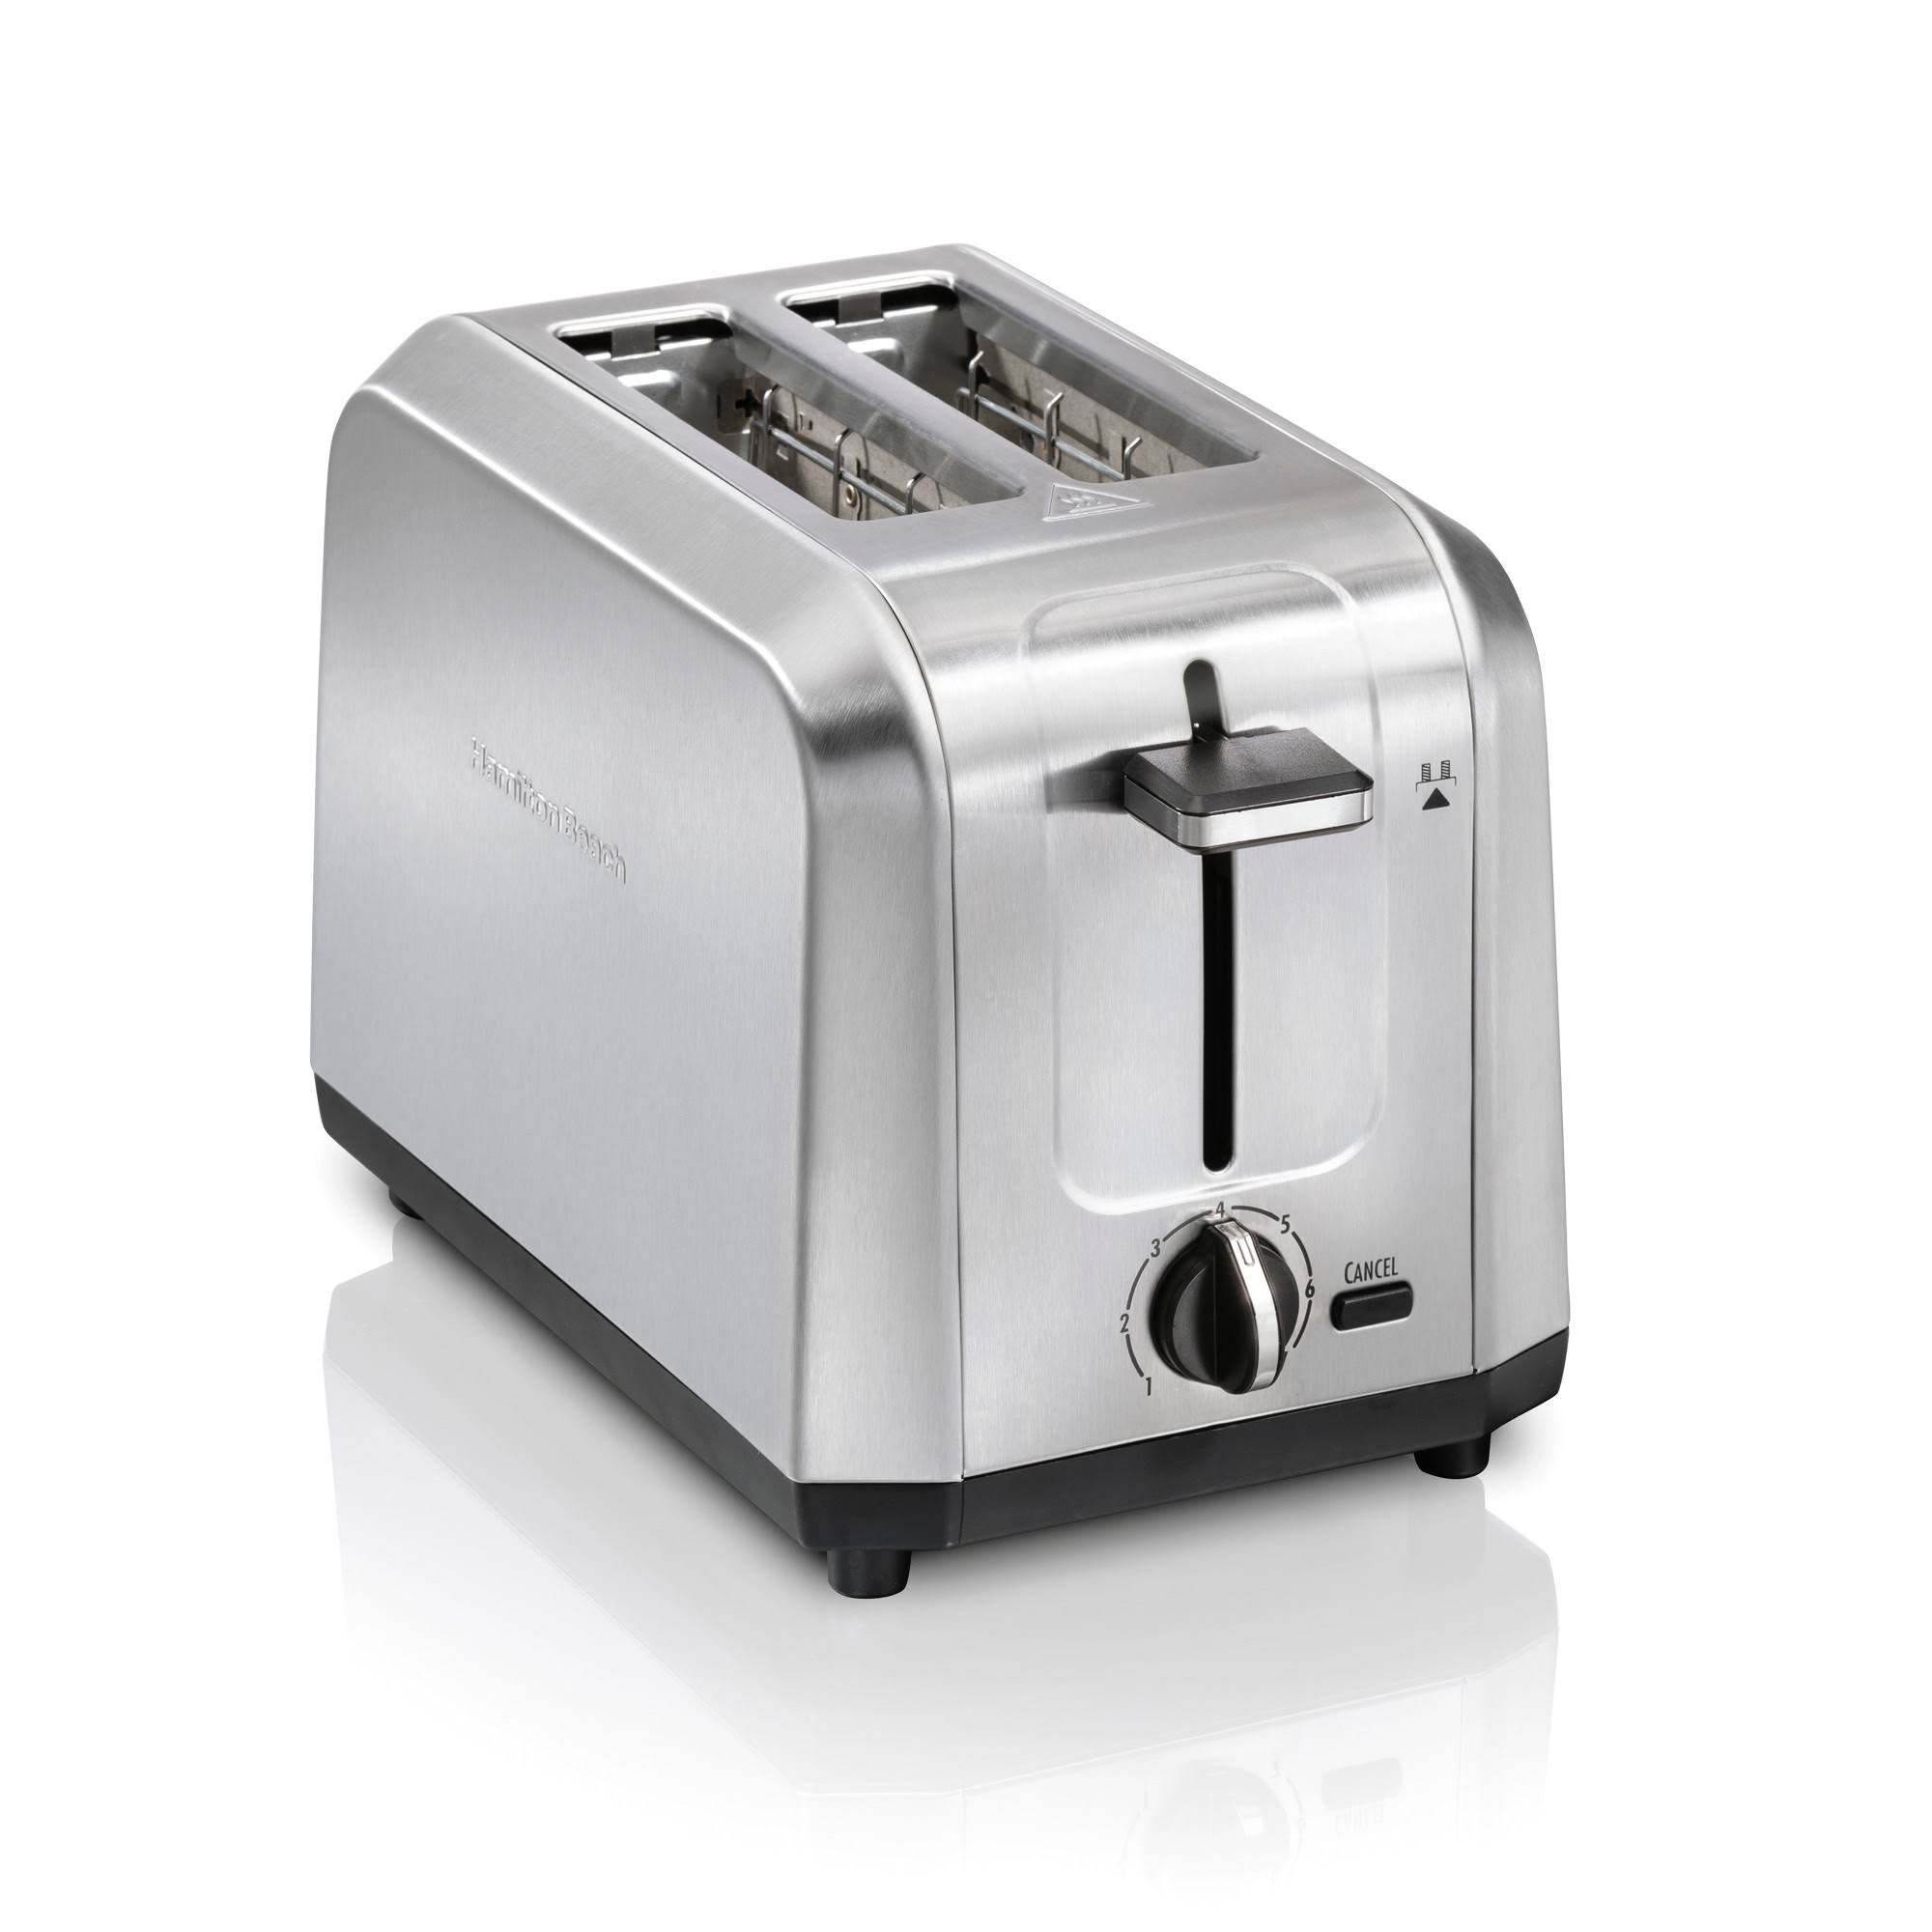
\includegraphics[scale=0.2]{toaster}
  \end{center}
  \caption{An example toaster.}
  \label{fig:toaster}
\end{figure}

The FRs are shown in Table \ref{toasterfrs}.  It is assumed that the design is either uncoupled or decoupled and
hence the independence of the FRs is as strong as possible.

\begin{table}[H]
  \centering
  \caption{Toaster Functional Requirements}
  \label{toasterfrs}
  \begin{tabular}{|c|l|}
    \hline
    \(\FR_1\) & Body contains all parts \\
    \hline
    \(\FR_2\) & Can be safely moved while hot \\
    \hline
    \(\FR_3\) & Can hold two slices of bread \\
    \hline
    \(\FR_4\) & Heats each slice of bread on both sides \\
    \hline
    \(\FR_5\) & Toasting is manually started \\
    \hline
    \(\FR_6\) & Toasting is automatically or can be manually stopped \\
    \hline
    \(\FR_7\) & Heat level can be controlled \\
    \hline
  \end{tabular}
\end{table}

The graph \(G_1\) for the first candidate design with \(n=7\) and \(m=13\) is shown in
\figurename~\ref{fig:design1}.

\begin{figure}[H]
  \centering
  \scalebox{0.75}{
    \begin{tikzpicture}
      \node [draw,circle] (fr1) at (4,0) {\(\FR_1\)};
      \node [draw,circle] (fr2) at (-1,2) {\(\FR_2\)};
      \node [draw,circle] (fr3) at (0,6) {\(\FR_3\)};
      \node [draw,circle] (fr4) at (1,2) {\(\FR_4\)};
      \node [draw,circle] (fr5) at (0,-4) {\(\FR_5\)};
      \node [draw,circle] (fr6) at (0,-1.5) {\(\FR_6\)};
      \node [draw,circle] (fr7) at (-4,0) {\(\FR_7\)};
      \draw (fr1) edge (fr3);
      \draw (fr1) edge (fr4);
      \draw (fr1) edge (fr5);
      \draw (fr1) edge (fr6);
      \draw (fr1) edge (fr7);
      \draw (fr2) edge (fr3);
      \draw (fr2) edge (fr4);
      \draw (fr2) edge (fr7);
      \draw (fr3) edge (fr4);
      \draw (fr3) edge (fr7);
      \draw (fr5) edge (fr6);
      \draw (fr5) edge (fr7);
      \draw (fr6) edge (fr7);
    \end{tikzpicture}
  }

  \(G_1\)
  \caption{First candidate design.}
  \label{fig:design1}
\end{figure}

Running the Bron Kerbosch and greedy last-first algorithms indicate that \(\X(G_1)=4\).  The \chromatic{4} coloring
returned by the greedy algorithm with:
\[C=\set{\text{\textcolor{green}{green}},\text{\textcolor{blue}{blue}},\text{\textcolor{red}{red}},
  \text{\textcolor{orange}{orange}}}\]
is show in \figurename~\ref{fig:d1color}.

\begin{figure}[H]
  \centering
  \scalebox{0.75}{
    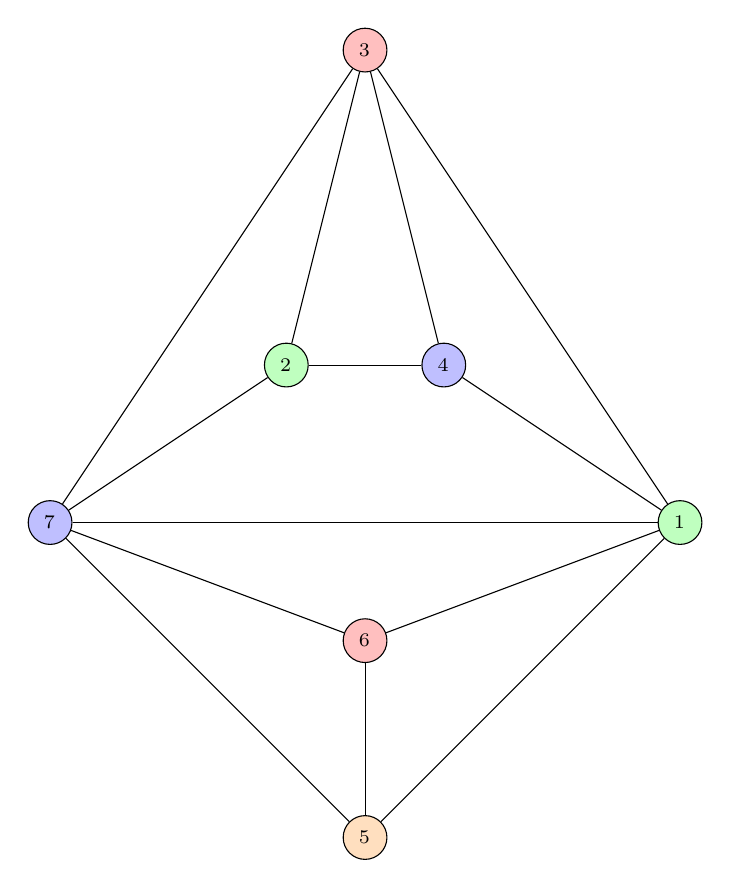
\begin{tikzpicture}
      \colorlet{c1}{green!25!white}
      \colorlet{c2}{blue!25!white}
      \colorlet{c3}{red!25!white}
      \colorlet{c4}{orange!25!white}
      \node [draw,circle,fill=c1] (fr1) at (4,0) {\(\FR_1\)};
      \node [draw,circle,fill=c1] (fr2) at (-1,2) {\(\FR_2\)};
      \node [draw,circle,fill=c3] (fr3) at (0,6) {\(\FR_3\)};
      \node [draw,circle,fill=c2] (fr4) at (1,2) {\(\FR_4\)};
      \node [draw,circle,fill=c4] (fr5) at (0,-4) {\(\FR_5\)};
      \node [draw,circle,fill=c3] (fr6) at (0,-1.5) {\(\FR_6\)};
      \node [draw,circle,fill=c2] (fr7) at (-4,0) {\(\FR_7\)};
      \draw (fr1) edge (fr3);
      \draw (fr1) edge (fr4);
      \draw (fr1) edge (fr5);
      \draw (fr1) edge (fr6);
      \draw (fr1) edge (fr7);
      \draw (fr2) edge (fr3);
      \draw (fr2) edge (fr4);
      \draw (fr2) edge (fr7);
      \draw (fr3) edge (fr4);
      \draw (fr3) edge (fr7);
      \draw (fr5) edge (fr6);
      \draw (fr5) edge (fr7);
      \draw (fr6) edge (fr7);
    \end{tikzpicture}
  }

  \(G_1\)
  \caption{First design chromatic coloring.}
  \label{fig:d1color}
\end{figure}

Notice in the design that \(\FR_5\) (start toasting) and \(\FR_6\) (stop toasting) have been forced into separate
parts, conceivably to accommodate the separate ``cancel'' button shown in \figurename~\ref{fig:toaster}.  But what
if the designer decides to eliminate the cancel button and allow manual cancellation via the lever?  Thus,
\(\FR_5\) and \(\FR_6\) no longer need to be separated, so the edge between their vertices can be eliminated.  The
result is shown in \figurename~\ref{fig:design2}.

\begin{figure}[H]
  \centering
  \scalebox{0.75}{
    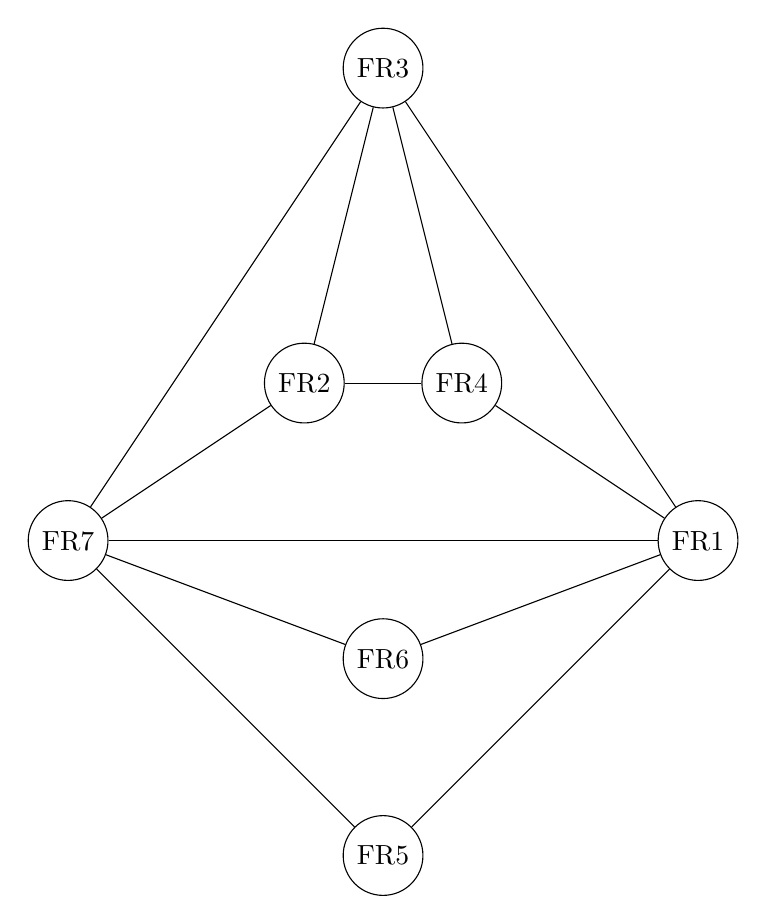
\begin{tikzpicture}
      \node [draw,circle] (fr1) at (4,0) {FR1};
      \node [draw,circle] (fr2) at (-1,2) {FR2};
      \node [draw,circle] (fr3) at (0,6) {FR3};
      \node [draw,circle] (fr4) at (1,2) {FR4};
      \node [draw,circle] (fr5) at (0,-4) {FR5};
      \node [draw,circle] (fr6) at (0,-1.5) {FR6};
      \node [draw,circle] (fr7) at (-4,0) {FR7};
      \draw (fr1) edge (fr3);
      \draw (fr1) edge (fr4);
      \draw (fr1) edge (fr5);
      \draw (fr1) edge (fr6);
      \draw (fr1) edge (fr7);
      \draw (fr2) edge (fr3);
      \draw (fr2) edge (fr4);
      \draw (fr2) edge (fr7);
      \draw (fr3) edge (fr4);
      \draw (fr3) edge (fr7);
      \draw (fr5) edge (fr7);
      \draw (fr6) edge (fr7);
    \end{tikzpicture}
  }

  \(G_2\)
  \caption{Second candidate design.}
  \label{fig:design2}
\end{figure}

Now, running the Bron Kerbosch and greedy last-first algorithms indicate that \(\X(G_1)=3\).  The \chromatic{3}
coloring returned by the greedy algorithm with:
\[C=\set{\text{\textcolor{green}{green}},\text{\textcolor{blue}{blue}},\text{\textcolor{red}{red}}}\]
is show in \figurename~\ref{fig:d2color}.

\begin{figure}[H]
  \centering
  \scalebox{0.75}{
    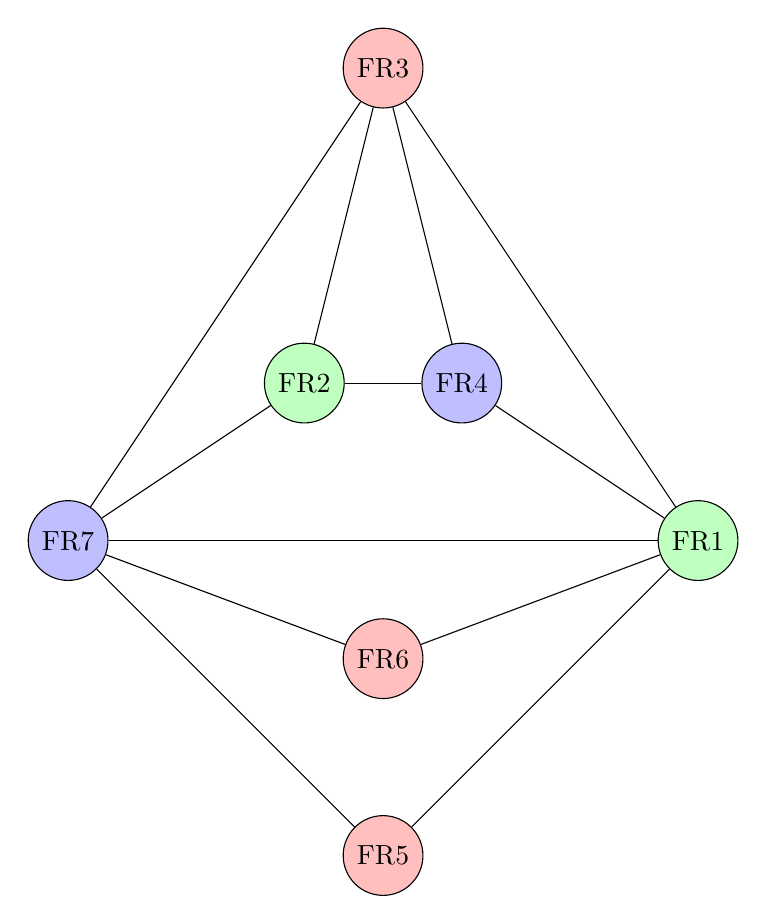
\begin{tikzpicture}
      \colorlet{c1}{green!25!white}
      \colorlet{c2}{blue!25!white}
      \colorlet{c3}{red!25!white}
      \node [draw,circle,fill=c1] (fr1) at (4,0) {FR1};
      \node [draw,circle,fill=c1] (fr2) at (-1,2) {FR2};
      \node [draw,circle,fill=c3] (fr3) at (0,6) {FR3};
      \node [draw,circle,fill=c2] (fr4) at (1,2) {FR4};
      \node [draw,circle,fill=c3] (fr5) at (0,-4) {FR5};
      \node [draw,circle,fill=c3] (fr6) at (0,-1.5) {FR6};
      \node [draw,circle,fill=c2] (fr7) at (-4,0) {FR7};
      \draw (fr1) edge (fr3);
      \draw (fr1) edge (fr4);
      \draw (fr1) edge (fr5);
      \draw (fr1) edge (fr6);
      \draw (fr1) edge (fr7);
      \draw (fr2) edge (fr3);
      \draw (fr2) edge (fr4);
      \draw (fr2) edge (fr7);
      \draw (fr3) edge (fr4);
      \draw (fr3) edge (fr7);
      \draw (fr5) edge (fr7);
      \draw (fr6) edge (fr7);
    \end{tikzpicture}
  }

  \(G_2\)
  \caption{Second design chromatic coloring.}
  \label{fig:d2color}
\end{figure}

This process gives the designer the feedback that the second design requires only three parts instead of four, and
thus has less information content and hence a higher chance of success than the first design.  It will be up to the
designer to weigh this result against other aspects of the design.

Note that in both cases, the chromatic number is equal to the lower and upper bounds.  In fact, the author found it
rather difficult to synthesis a case study with meaningful relationships between the FRs such that this was not the
case.  The random graph analysis supports this, with such a high percentage of the random graphs exhibiting this
quality.
